\section{Graph Energies}
\begin{frame}{Graph Energies}
\begin{itemize}
    \item The graph energy, on a connected finite graph G, is defined as
    \begin{equation}
        E_G(u):=\underset{x \thicksim y}{\sum}\left(u(x)-u(y)\right)^2
    \end{equation}
    
    \item It is a quadratic form in $u$ associated to the following bilinear form
    \begin{equation}
        E_G(u,v):= \underset{x\thicksim y}{\sum}\left(u(x)-u(y)\right)\left(v(x)-v(y)\right)
    \end{equation}
\end{itemize}

Let's denote by $G:=(V,E)$, where
$$
\left\{
\begin{array}{rcl}
   V= &\text{ \,set of vertices}  \\
   E= &\text{ set of edges}.
\end{array}\right.
$$
\end{frame}
\begin{frame}{Markov Property (Compatibility with  with normal contraction)}
\begin{itemize}
    \item If $u:V \rightarrow \mathbb{R}_+$, we denote by $[u]=\min\{1,u\vee 0\}$. Then the energy $E_G(\cdot)$ satisfies the so called \textbf{Markov Property}, which is
    \begin{equation}
    E_G([u])\leq E_G(u).
    \end{equation}
    \item Let $G':=(V',E')$ such that $G\subseteq G'$ is a sub-graph. For $u:V \rightarrow \mathbb{R}_+$ given, $\,\,\exists$ $\tilde{u}: V' \rightarrow \mathbb{R}$ such that $\tilde{u}\lvert_V=u$ and that 
    $$
\underset{u'\lvert_V=u}{\inf}E_{G'}(u')=E_{G'}(\tilde{u})
    $$
\item $\tilde{u}$ is called the \textbf{harmonic extension}

\item For all examples of interest to us ($I$ and $SG$ included) we have
\begin{equation}
    E_{G'}(\tilde{u})=r\,E_G(u) \quad \text{ for all } u: V \rightarrow \mathbb{R}.
\end{equation}
for some $r\in (0.1)$. This called the \textbf{renormalization equation}.
\end{itemize}
\end{frame}

\begin{frame}
Therefore we have
\begin{equation}
    \frac{1}{r}\,E_{G'}(u')\geq E_G(u).
\end{equation}
This means that energy increase with \textbf{general extension}, except in the case of harmonic extension where the energy is \textbf{constant}.
\begin{example}
    Let's consider $K=SG$ and suppose $u(\cdot)$ is defined on $V_0$ by 
$$
\left\{
\begin{array}{rcl}
   u(q_0)=a  \\
   u(q_1)=b&.\\
   u(q_0)=c&
\end{array}\right.
$$
Then 

\begin{align*}
    E_1(\tilde{u})&=(a-z)^2+(b-z)^2+(b-x)^2+(c-x)^2+\\
    &+(a-y)^2+(c-y)^2+ (x-y)^2+(z-y)^2+(x-z)^2.
\end{align*}
is to be minimized.
\end{example}
\end{frame}
\begin{frame}
\begin{figure}
\centering
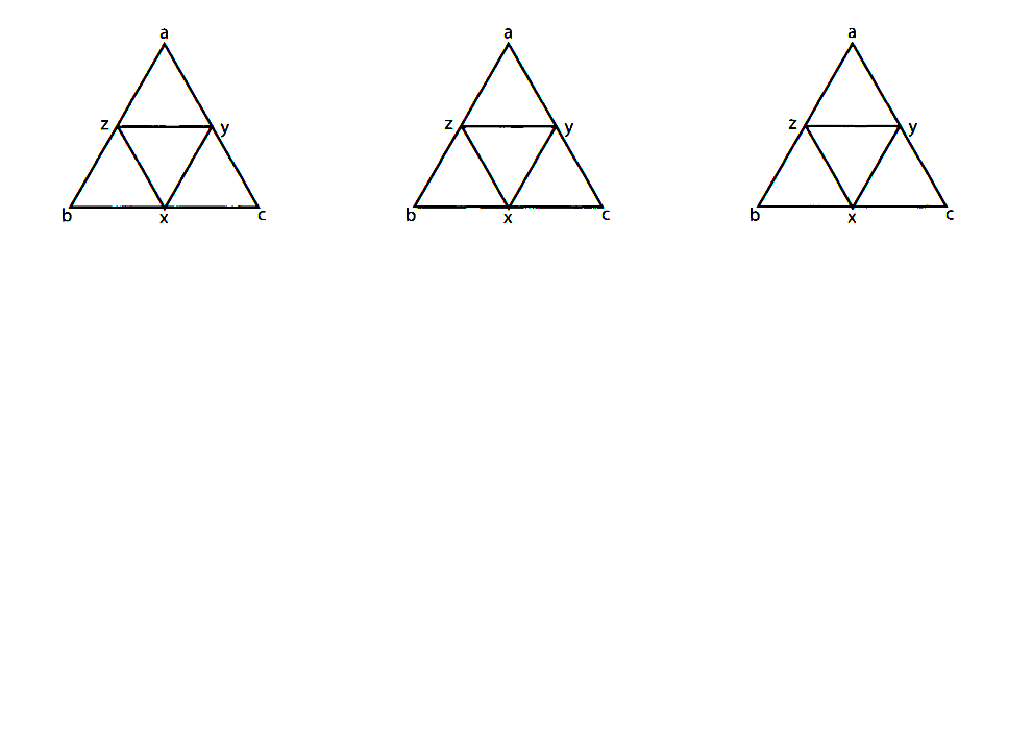
\includegraphics[height=5em]{images/harmonic extension order 1.pdf}
\caption{harmonic extension on $V_1$}
\end{figure}

\begin{itemize}
\item By calculating partial derivatives on x,y and z, we obtain 
\begin{align}\label{1st harm extension}
    %\begin{aligned}
    \left\{ \begin{array}{rcl}
        u(F_0q_1)=u(F_1q_0)=x:=& {\color{red} \frac{1}{5}}.a+{\color{blue} \frac{2}{5}}.b+{\color{blue} \frac{2}{5}}.c \\
        \\
        u(F_0q_2)=u(F_2q_0)=y:=& {\color{blue} \frac{2}{5}}.a+{\color{red} \frac{1}{5}}.b+{\color{blue} \frac{2}{5}}.c \\
        \\
        u(F_1q_2)=u(F_2q_1)=z:=& {\color{blue} \frac{2}{5}}.a+{\color{blue} \frac{2}{5}}.b+{\color{red} \frac{1}{5}}.c \\
    \end{array}\right.
    %\end{aligned}
\end{align}

\item In the particular \textbf{symetric} case, i.e. when $a=1$ and $b=c=0$, we obtain $x=1/5$ and $y=z=2/5$. 
\end{itemize}
\end{frame}
\begin{frame}
\begin{itemize}
    \item Using \eqref{1st harm extension}, we can show easily that 
    \begin{align}
        E_1(\tilde{u})=r.E_0(u),
    \end{align}
    where $r=3/5$, so the \textbf{renormalized energy} is given by:
    $$
    \mathcal{E}_{1}(\tilde{u}):=r^{-1}E_1(\tilde{u})=E_0(u).
    $$
\item $\tilde{u}$ is the \textbf{harmonic extension} from $V_1$ to $V_2$.

\item The same idea could be done, for $u:V_m\rightarrow \mathbb{R}$ given, to obtain the \textbf{harmonic extension} form $V_m$ to $V_{m+1}$ such that:
\begin{align}
    \left\{ \begin{array}{cc}
        &E_{m+1}(\tilde{u})=r.E_{m}(u)   \\
        &\mathcal{E}_{m+1}(\tilde{u})=r^{-1}E_{m}(u) 
    \end{array}\right.
\end{align}
\end{itemize}    
\end{frame}
\begin{frame}
    \begin{itemize}
        \item If $u:V_m\rightarrow \mathbb{R}$ is given and $u':V_{m+1}\rightarrow \mathbb{R}$ to be any arbitrary extension, then 
        \begin{align}
        E_{m+1}(u')=\underset{|\omega|=m}{\sum}E_1(u'\circ F_{\omega})    
        \end{align}
        and 
        \begin{align}
        E_{m+1}(u')=\underset{i=0,1,2}{\sum}E_m(u'\circ F_{i})    
        \end{align}
        
        \item The renormalized energy 
        $$
        \mathcal{E}_{m}(u)=(3/5)^{-m}\,E_{m}(u).,
        $$
        is constant under the harmonic extension. Moreover, it's a nondecreasing sequence for any extension. i.e.
        \begin{align}
            \mathcal{E}_{0}(u)\leq \mathcal{E}_{1}(u)\leq \ldots.
        \end{align}
    \end{itemize}
\end{frame}
\begin{frame}{Summary}
    TO summarize: Let $u$ be a function on $V_m$, then the harmonic extension $\tilde{u}$ to $V_{m+1}$ may be characterized in three ways:
    \vspace{0.25cm}
\begin{itemize}
    \item[(i)] it minimizes $\mathcal{E}_{m+1}(\tilde{u})$ at the value $\mathcal{E}_m(u)$;
    \item[(ii)] at each new point $x \in V_{m+1} \backslash V_m, \tilde{u}(x)$ is \textbf{the average of the values at the four neighboring points in} $V_{m+1}$; i.e. 
    $$
\tilde{u}(x)=\dfrac{1}{4}\underset{\substack{y \in V_{m+1} \\ y \underset{m+1}{\thicksim} x}}{\sum}\tilde{u}(y)
    $$
    \item[(iii)] it satisfies the " $\frac{1}{5}-\frac{2}{5}$ rule" at the new points in $V_{m+1} \backslash V_m$. 
\end{itemize}
\end{frame}
\section{Energy}
\begin{frame}{Energy}
\begin{itemize}
\item Since, for any function $u$ on $V_*$, the sequence of energies $\mathcal{E}_{m}(u)$ is nondecreasing. It make sense to define 
$$
\mathcal{E}(u):=\lim_{m\rightarrow +\infty}\mathcal{E}_{m}(u).
$$

\item Moreover 
\begin{align}\label{when energy vanish}
\mathcal{E}(u)=0 \quad \Leftrightarrow \quad u=cts, 
\end{align}
and 
\begin{align}\label{dom energy}
\operatorname{dom}(\mathcal{E})=\left\{ u:V_*\rightarrow \mathbb{R}\,:\,\, \mathcal{E}(u)<\infty \right\}.
\end{align}
\end{itemize}
\end{frame}
\begin{frame}{Consequences}
\begin{itemize}
\item Let $u:V_*\rightarrow \mathbb{R}$ such that $\mathcal{E}(u)<\infty$. Therefore
\begin{align}
\lvert u(x)-u(y)\rvert\leq r^{m/2}\,\mathcal{E}^{1/2}(u)\quad \text{for all } x\underset{m}{\thicksim} y\in V_m.
\end{align}

\vspace{0.25cm}
\item From the geometry of $K$ (either I or SG) it can be seen that if $x,y\in V_*$ belong to the \textbf{same} or \textbf{adjacent} $m$-cell, with some technical calculation, we obtain 
\begin{align}\label{mod-cont}
\lvert u(x)-u(y)\rvert  \leq \frac{r^{m/2}}{1-r^{1/2}}\, \mathcal{E}^{1/2}(u).
\end{align}

\item When $K=I$ is the \textbf{interval}, \eqref{mod-cont} ensures that $u$ is $1/2$-Hölder continuous. Precisely; since $r=1/2$, if $x,y$ are suc that $|x-y|\leq 1/2^{m}$ then $x$ and $y$ belongs to the same or adjacent $m$-cell. Hence \eqref{mod-cont} ensures that
\begin{equation}
    |u(x)-u(y)|\leq M |x-y|^{1/2}.
\end{equation}
%\item Moreover, for $x_m,x_{m+1},\ldots,x_{m+k}$ such that 
%$$
%\left\{\begin{array}{cc}
%& x_{m+j}\in V_{m+j}  \\
%& x_{m+j}\underset{m+j+1}{\thicksim} x_{m+j+1}
%\end{array}\right.,
%$$
%then 
%\begin{align}
%\lvert u(x_m)-u(x_{m+k})\rvert & \leq r^{m/2}\left(1+r^{1/2}+\ldots+r^{k/2}\right)\,\mathcal{E}^{1/2}(u)\nonumber \\
%& \leq \frac{r^{m/2}}{1-r^{1/2}}\, \mathcal{E}^{1/2}(u).
%\end{align}
\end{itemize} 
\end{frame}

\begin{frame}
\begin{itemize}
\item When $K=SG$, the $1/2$-Hölder continuity can be obtained in \textbf{another metric}, called the \textbf{resistance metric}, which we denote by $R(\cdot,\cdot)$. Hence if $u\in \operatorname{dom}(\mathcal{E})$ then for all $m\geq 1$
\begin{equation}
    \lvert u(x)-u(y)\rvert \leq M\cdot R(x,y)^{1/2}, 
\end{equation}
for all $x,y \in K$ such that $R(x,y)\leq r^{m}$.

\item Moreover, this resistance metric $R(\cdot,\cdot)$ is equivalent to the Euclidean metric with some exponent $0<\beta<1$, i.e. 
\begin{equation}
R(x,y)\thicksim \lVert x-y \rVert^{\beta} \quad \text{ for } \quad \beta=\log \frac{5}{3}/\log 2. 
\end{equation}
\end{itemize}
\end{frame}

\begin{frame}{Hilbert space property/Self-Similarity of the energy}
\begin{theorem}
    $dom(\mathcal{E})/constants$ forms a Hilbert space with the inner product given by 
    \begin{equation}\label{inner prod}
        (u,v)_{\mathcal{E}}:=\mathcal{E}(u,v):=\lim_{m\rightarrow \infty}\mathcal{E}_m(u,v) \quad \text{ for all } u,v \in \operatorname{dom}(\mathcal{E})
    \end{equation}
\end{theorem}
The next result expresses the self-similarity of the energy.
\begin{theorem}
If $u \in \operatorname{dom}(\mathcal{E})$ then $u \circ F_i \in \operatorname{dom}(\mathcal{E})$ for all $i$, and
\begin{align}\label{self-sim energy}
    \mathcal{E}(u)=\sum_i r^{-1} \mathcal{E}\left(u \circ F_i\right)
\end{align}
\end{theorem}
\end{frame}

\begin{frame}
This self-similarity of the energy follows from the following fact
$$
\mathcal{E}_{m+1}(u)=\sum_{i=0}^{2} r^{-1} \mathcal{E}_m\left(u \circ F_i\right).
$$
Moreover, for any partition $\mathcal{P}$, using the subdivision:
\begin{equation}
    K=\underset{\omega \in \mathcal{P}}{\bigcup}F_{\omega}K,
\end{equation}
and replacing $r^{-1}$ by $r^{-|\omega|}$, we obtain
\begin{align}\label{self-sim energy}
    \mathcal{E}(u)=\sum_{\omega\in \mathcal{P}} r^{-|\omega|} \mathcal{E}\left(u \circ F_{\omega}\right).
\end{align}
\end{frame}
\begin{frame}{Self-Similar measure}
\begin{itemize}
    \item The previous self-similarity equation suggest the existence of a measure $\nu_u$ defined through energies. More precisely, we have
    $$
    \nu_u\left(F_{\omega} K\right):=r^{-|\omega|} \mathcal{E}\left(u \circ F_{\omega}\right).
    $$
    \item Equivalently, we can check that 
    $$
    \nu_{u}(F_{\omega}K)=\lim_{m\rightarrow \infty}r^{-m}\underset{x \underset{m}{\thicksim} y\,\,:\,\,x,y\in F_{\omega}K}{\sum}\left(u(x)-u(y)\right)^{2}.
    $$
    \item It can be shown that, for all $u\in \operatorname{dom} \mathcal{E}$ we have 
    $$
    \nu_{u}\left(F_{\omega}K\right)\leq r^{|\omega|}\mathcal{E}(u)\quad \text{ for all } \omega \in \mathcal{P} .
    $$
\end{itemize}
\end{frame}
\begin{frame}{Markov property/Compatibility with normal contraction}
    \begin{itemize}
    \item The {Markov property/Compatibility with normal contraction} holds for all $u\in \operatorname{dom}(\mathcal{E})$, i.e.
    $$
    \mathcal{E}([u])\leq \mathcal{E}(u), 
    $$
    where $[u]=min\{1, u\vee 0\}$.
    \end{itemize}
\end{frame}
